%\documentclass[journal]{IEEEtran}
%\documentclass[11pt, a4paper, oneside]{article}
\documentclass[11pt, a4paper, oneside]{article}

\usepackage{appendix}

% Incluimos el paquete Babel que sirve para separar correctamente las palabras de multitud de idiomas.
\usepackage[spanish]{babel}

% Este paquete permite poner acentos directamente.
%:
\usepackage[latin1]{inputenc}

\usepackage[T1]{fontenc}

\usepackage{comment}

% Macros AMS para teoremas.
\usepackage{amsmath}

% Romper autom�ticamente ecuaciones muy largas
%\usepackage{breqn}

% Permite usar fuentes AMS.
\usepackage{amsfonts}

% Para usar s�mbolos AMS.
\usepackage{amssymb}

% ?
\usepackage{color}
\definecolor{gray}{rgb}{0.4,0.4,0.4}
\definecolor{darkblue}{rgb}{0.0,0.0,0.6}
\definecolor{cyan}{rgb}{0.0,0.6,0.6}

% Color en las tablas.
\usepackage{colortbl}

% Para usar el s�mbolo del euro.
\usepackage{eurosym}

%?
\usepackage{listings}

% ?
\usepackage{mathrsfs}

% Uso desconocido.
\usepackage{shadow}

% Espaciado de primera l�nea de cada p�rrafo.
\usepackage{indentfirst}

% ?
\usepackage{theorem}

% ?
\usepackage{shadow}

% Permite un manejo sencillo de los ap�ndices. Permite tambi�n introducir subapendices.
%\usepackage{appendix} 

%?
\usepackage[pdftex]{graphicx}

% De esta forma aparecen hiperv�nculos en el PDF.
\usepackage[colorlinks=true]{hyperref}

% Soporte para el comando \marginsize.
\usepackage{anysize} 

%Permite manejar los m�rgenes de forma sencilla.
\marginsize{3cm}{2cm}{2.5cm}{2.5cm}

\usepackage{url}

% Usado junto con \begin{figure}[H] ... pone la figura exactamente donde yo quiero.
\usepackage{float}

\usepackage[mediumspace,mediumqspace,squaren,binary]{SIunits}
%\sisetup{per-mode=symbol,per-symbol = p}
%\usepackage{siunitx}
%\sisetup{per-mode=symbol,detect-all}
%\usepackage{xfrac}
%\sisetup{per-mode=fraction,fraction-function=\sfrac,alsoload=binary}

%?
\usepackage{subfigure}

%?
\usepackage{verbatim}

% Permite usar el s�mbolo de euro.
%\usepackage{eurofont}

% ?
%\addtolength{\footskip}{+3cm}

% Para un encabezado especial m�s visual usar
%\usepackage{fancyhdr} y \pagestyle{fancy}             

% Para que el nombre del capitulo salga m�s chulo.
\usepackage[Lenny]{fncychap}
\usepackage{fancyvrb}


% ?
\usepackage{extramarks}

% Para poder intercalar imagen y texto.
\usepackage{wrapfig} 
\usepackage{multicol}
\usepackage{rotating}
\setlength\unitlength{1mm}

\linespread{1.5}

\DeclareMathOperator*{\argmax}{arg\,max}
\DeclareMathOperator*{\argmin}{arg\,min}

% Declare the extension of the images you are going to use, so you won't have to specify these with
% every instance of \includegraphics
\DeclareGraphicsExtensions{.jpg, .pdf, .mps, .png, .gif, .fig, .bmp}

% Declare the path(s) where your graphic files are
\graphicspath{{../1_Figuras/}}


\makeatletter
\renewcommand{\paragraph}{\@startsection{paragraph}{4}{0ex}%
   {-3.25ex plus -1ex minus -0.2ex}%
   {1.5ex plus 0.2ex}%
   {\normalfont\normalsize\bfseries}}
\makeatother

\stepcounter{secnumdepth}
\stepcounter{tocdepth}


%%%%%%%%%%%%%%%%%%%%%%
%%%%%%%%%%%%%%%%%%%%%%
%%%%%%%%%%%%%%%%%%%%%%

% COMIENZA EL DOCUMENTO

%%%%%%%%%%%%%%%%%%%%%%
%%%%%%%%%%%%%%%%%%%%%%
%%%%%%%%%%%%%%%%%%%%%%

\begin{document}

%%%%%%%%%%%%%%%%%%%%%%
%%%%%%%%%%%%%%%%%%%%%%
%%%%%%%%%%%%%%%%%%%%%%

% TITULO

%%%%%%%%%%%%%%%%%%%%%%
%%%%%%%%%%%%%%%%%%%%%%
%%%%%%%%%%%%%%%%%%%%%%

\title{Robot's trajectories based on the speed of the wheels}
\maketitle

\noindent $\omega_l$ is the left wheel's angular velocity expressed in radians/seconds.\\  
$\omega_r$ is the right wheel's angular velocity expressed in radians/seconds.\\ 
$r$ is the wheel's radius expressed in meters.\\  
$L$ is the distance between wheels expressed in meters.\\  
$T$ is the movement time.\\

\noindent The most general trajectory that a robot can describe when the speed of the wheels are different (different in magnitude and sign), and remain constant for $T$ seconds, is a circumference of radius $R$. This trajectory can be simplified depending of how these speeds are related.\\

\noindent In the next section the equations for the most general case are derived. A graph is provided for clarity purposes. In the graph it has been considered:  
\[\omega_l~!=~\omega_r\]  
with $\omega_l$ and $\omega_r$ positive, so the robot moves forwards.\\

\noindent (NOTE: These equations works for every possible value of $\omega_l$ and $\omega_r$, but for clarity issues I chose positive values for the speed of the wheels in order to get the robot moves forwards in the graph.)

\noindent Linear velocity of each wheel.  
%ECUACI�N{
\begin{align}
v_l &= \omega_l \cdot r\\
v_r &= \omega_r \cdot r 
\label{Eq:vlvr}
\end{align}
%}

\noindent Turned angle for each wheel after T seconds.  
%ECUACI�N{
\begin{align}
\theta_l &= \omega_l \cdot T\\  
\theta_r &= \omega_r \cdot T  
\label{Eq:tltr}
\end{align}
%}

%FIGURA{
\begin{figure}[H]
 \begin{center}
  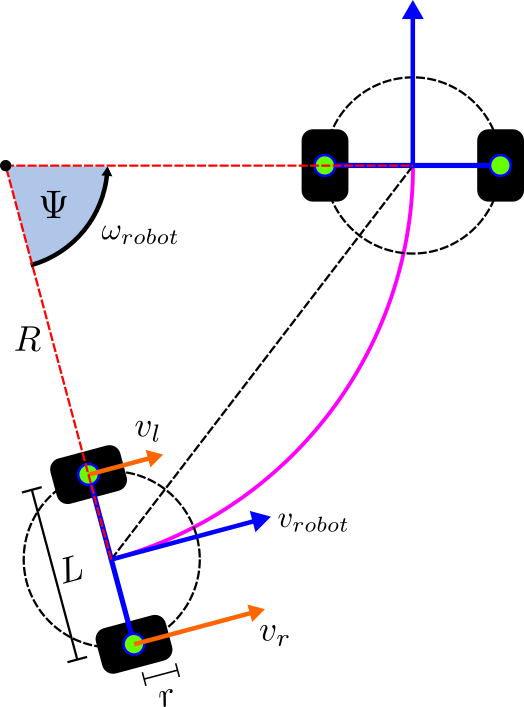
\includegraphics[scale=1.5]{Trajectories.png}
  \caption{General trajectory}
  \label{fig:circumference}
 \end{center}
\end{figure}
%}

\noindent Traveled distance for each wheel after T seconds.  
%ECUACI�N{
\begin{align}
D_l &= \theta_l \cdot r = \omega_l \cdot T \cdot r = v_l \cdot T\\
D_r &= \theta_r \cdot r = \omega_r \cdot T \cdot r = v_r \cdot T
\label{Eq:dldr}
\end{align}
%}

\noindent Turned angle by the robot after T seconds.  
%ECUACI�N{
\begin{align}
\psi = \omega_{robot} \cdot T
\label{Eq:psi}
\end{align}
%}

\noindent Arcs subtending the $\psi$ angle for each wheel after T seconds.  
%ECUACI�N{
\begin{align}
A_{l} = \psi \cdot \left(R - \frac{L}{2} \right) = \omega_{robot} \cdot T \cdot \left( R - \frac{L}{2} \right)\\
A_{r} = \psi \cdot \left(R + \frac{L}{2} \right) = \omega_{robot} \cdot T \cdot \left( R + \frac{L}{2} \right)
\label{Eq:alar}
\end{align}
%}


\noindent Each wheel has traveled a distance $D_x$ which is associated to the corresponding arc $A_x$, where $x=\left\{l, r\right\}$
%ECUACI�N{
\begin{align}
A_l &= D_l\\
A_r &= D_r
\label{Eq:alar2}
\end{align}
%}

%ECUACI�N{
\begin{align}
\omega_{robot} \cdot T \cdot \left(R + \frac{L}{2} \right) &= \omega_r \cdot T \cdot r
\label{Eq:wr}
\end{align}
%}

%ECUACI�N{
\begin{align}
\omega_{robot} \cdot T \cdot \left(R -\frac{L}{2} \right) &= \omega_l \cdot T \cdot r
\label{Eq:wl}
\end{align}
%}

\noindent If \ref{Eq:wr} and \ref{Eq:wl} are added:
%ECUACI�N{
\begin{align}
2 \cdot \omega_{robot} \cdot R = \left( \omega_r + \omega_l\right) \cdot r
\label{Eq:wrobot}
\end{align}
%}
  
\noindent Using the following expression
%ECUACI�N{
\begin{align}
v_{robot} = \omega_{robot} \cdot R
\label{Eq:vrobot}
\end{align}
%}

\noindent the equation for the robot's linear velocity is obtained:
%ECUACI�N{
\begin{align}
v_{robot} = \frac{\left(\omega_r + \omega_l\right) \cdot r}{2} = \frac{v_r + v_l}{2}
\label{Eq:vrobot2}
\end{align}
%}

\noindent If \ref{Eq:wr} and \ref{Eq:wl} are subtracted:
%ECUACI�N{
\begin{align}
\omega_{robot} \cdot L = \left(\omega_r - \omega_l\right) \cdot r
\label{Eq:wrobot2}
\end{align}
%}

%ECUACI�N{
\begin{align}
\omega_{robot} = \frac{\left(\omega_r - \omega_l\right) \cdot r}{L} = \frac{v_r - v_l}{L}
\label{Eq:wrobot3}
\end{align}
%}

\noindent An expression for the turn radius is derived using the previous results:
%ECUACI�N{
\begin{align}
R = \frac{v_{robot}}{\omega_{robot}} = \frac{L}{2}\cdot\frac{\left(\omega_r+\omega_l\right)}{\left(\omega_r - \omega_l\right)}
\label{Eq:R}
\end{align}
%}

\noindent Finally, an expression for $\psi$ is obtained using the turned angle for each wheel after T seconds.
%ECUACI�N{
\begin{align}
\psi = \omega_{robot} \cdot T = \frac{r}{L}\left(\omega_r - \omega_l\right) \cdot T = \frac{r}{L}\left(\theta_r - \theta_l\right)
\label{Eq:psi}
\end{align}
%}

\noindent Equations summary:
%ECUACI�N{
\begin{align}
v_{robot} &= \frac{v_r + v_l}{2} = \frac{\left(\omega_r + \omega_l\right) \cdot r}{2}\\
\omega_{robot} &= \frac{v_r - v_l}{L} = \frac{\left(\omega_r - \omega_l\right) \cdot r}{L}\\
R &= \frac{v_{robot}}{\omega_{robot}} = \frac{L}{2}\cdot\frac{\left(\omega_r+\omega_l\right)}{\left(\omega_r - \omega_l\right)}\\
\psi &= \omega_{robot} \cdot T = \frac{r}{L}\left(\theta_r - \theta_l\right) = \frac{r}{L}\left(\omega_r - \omega_l\right) \cdot T
\label{Eq:vrobot4}
\end{align}
%}

\noindent Reverse equations summary:
%ECUACI�N{
\begin{align}
\omega_r &= \frac{2 \cdot v_{robot} + L \cdot \omega_{robot}}{2 \cdot r}\\
\omega_l &= \frac{2 \cdot v_{robot} - L \cdot \omega_{robot}}{2 \cdot r}
\label{Eq:wrwl2}
\end{align}
%}

\noindent Examples:

\begin{itemize}
\item The robot moves in straight line if $\omega_l = \omega_r$. If $\omega_l > 0$ rad/sec the robot moves forwards. If $\omega_l < 0$ rad/sec the robot moves backwards. A straight line is a circumference with infinite radius.\\
$\omega_l = \omega_r = 0.2$ rad/sec. $T=2$ sec. $r=10$ cm and $L=30$ cm.
%ECUACI�N{
\begin{align}
v_{robot} &= 2~\mbox{cm/s}\\
\omega_{robot} &=0~\mbox{rad/sec}\\
R_{robot} &=\infty~\mbox{cm}\\
\psi &= 0 ~\mbox{cm}
\end{align}
%}

\item The robot rotates around itself if $\omega_l = -\omega_r$. If $\omega_l > 0$ rad/sec the robot rotates to the right (clockwise). If $\omega_l < 0$ rad/sec the robot rotates to the left (counterclockwise).\\
$\omega_l = 0.2$ rad/sec. $\omega_r = -0.2$ rad/sec. $T=2$ sec. $r=10$ cm and $L=30$ cm.
%ECUACI�N{
\begin{align}
v_{robot} &= 0~\mbox{cm/s}\\
\omega_{robot} &=-0.13~\mbox{rad/sec}~(-7.44�/seg)\\
R_{robot} &=0 ~\mbox{cm}\\
\psi &= -0.26~\mbox{rad}~(-14.89�)
\end{align}
%}

\item The robot describes a circumference of radius R if $\omega_l~!=~\omega_r$. If $\omega_l > \omega_r > 0$ rad/sec the robot rotates to the right (clockwise). If $\omega_r > \omega_l > 0$ rad/sec the robot rotates to the left (counterclockwise).\\
$\omega_l = 0.1$ rad/sec. $\omega_r = 0.2$ rad/sec. $T=2$ sec. $r=10$ cm and $L=30$ cm.
%ECUACI�N{
\begin{align}
v_{robot} &= 1.5~\mbox{cm/s}\\
\omega_{robot} &=0.03~\mbox{rad/sec}~(1.94�/seg)\\
R_{robot} &=45~\mbox{cm}\\
\psi &= 0.06~\mbox{rad}~(3.81�)
\end{align}
%}

\end{itemize}

%FIGURA{
\begin{figure}[H]
 \begin{center}
  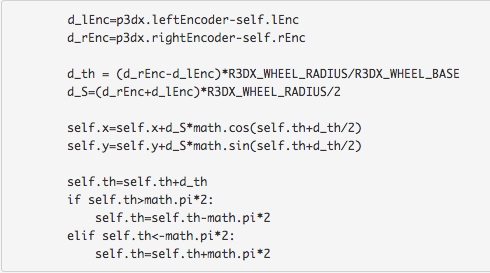
\includegraphics[scale=0.8]{Odometry.png}
  \caption{Odometry equations}
  \label{fig:odometry}
 \end{center}
\end{figure}
%}

\end{document}
